\documentclass[twoside]{article}
\usepackage[utf8]{inputenc}
\usepackage{amsmath,amsfonts,amssymb,amsthm,latexsym}
\usepackage[spanish,es-noshorthands]{babel}
\usepackage[T1]{fontenc}
\usepackage{lmodern}
\usepackage{graphicx,hyperref}
\usepackage{tikz,pgf}
\usepackage{marvosym}
\usepackage{multicol}
\usepackage{fancyhdr}
\usepackage[papersize={5.5in,8.5in},left=.75cm,right=.75cm,top=1.5cm,bottom=1.25cm]{geometry}
\usepackage{fancyhdr}
\pagestyle{fancy}
\fancyhead[LE]{Colegio Arborizadora Baja}
\fancyhead[RE]{PEI:``Hacia una cultura para el desarrollo sostenible''}
\fancyfoot[RO]{\Email iedabgerman@autistici.org}
\fancyhead[LO]{\url{www.autistici.org/mathgerman}}
\fancyfoot[RE]{\Email cedarborizadoraba19@redp.edu.co}
\fancyfoot[LE]{Calle 59I \#44A - 02 \Telefon 7313994 - 7313995}
\fancyhead[RO]{Nit 830024976-8, Código DANE 11100103084-8}

\author{Germ\'an Avenda\~no Ram\'irez~\thanks{Lic. Mat. U.D., M.Sc. U.N.}}
\title{\begin{minipage}{.2\textwidth}

\includegraphics[height=1.75cm]{Images/logo-colegio.png}\end{minipage}
\begin{minipage}{.55\textwidth}
\begin{center}
Porcentajes\\
Aritmética $7^{\circ}$
\end{center}
\end{minipage}\hfill
\begin{minipage}{.2\textwidth}

\includegraphics[height=1.75cm]{Images/logo-sed.png} 
\end{minipage}}
\date{}
\thispagestyle{plain}
\begin{document}
\maketitle
%Nombre: \hrulefill Curso: \underline{\hspace*{44pt}} Fecha: \underline{\hspace*{2.5cm}}
\begin{minipage}{.95\textwidth}
\fbox{\textit{No raye ni dañe esta hoja para que pueda usarla otro compañero}}
\end{minipage}
\subparagraph*{A.} Encuentre el área sombreada en notación de porcentaje.
\begin{enumerate}
\begin{multicols}{3}
\item \begin{tikzpicture}[scale=.25]
\filldraw[gray!30] (0,5) rectangle (3,10);
\filldraw[gray!30] (4,0) rectangle (5,3);
\draw (0,0) grid (10,10);
\end{tikzpicture}
\item \begin{tikzpicture}[scale=.25]
\filldraw[gray!30] (0,5) rectangle (3,10);
\filldraw[gray!30] (2,0) rectangle (3,1);
\filldraw[gray!30] (3,0) rectangle (10,10);
\draw (0,0) grid (10,10);
\end{tikzpicture}
\item \begin{tikzpicture}[scale=.25]
\filldraw[gray!30] (0,3) rectangle (10,4);
\filldraw[gray!30] (2,2) rectangle (7,3);
\filldraw[gray!30] (4,4) rectangle (8,5);
\draw (0,0) grid (10,10);
\end{tikzpicture}
\end{multicols}
\subparagraph*{B.} Escriba de tres maneras diferentes cada porcentaje
\begin{multicols}{4}
\item 90\%
\item 58.7\%
\item 12.5\%
\item 130\%
\end{multicols}
\subparagraph*{C.} Encuentre la notación decimal correspondiente
\begin{multicols}{4}
\item 67\%
\item 45\%
\item 59.01\%
\item 10\%
\item 1\%
\item 200\%
\item 0.1\%
\item 0.09\%
\item 0.18\%
\item 23.19\%
\item $14\frac{7}{8}$\%
\item $56\frac{1}{2}$\%
\end{multicols}
\subparagraph*{D.} Escriba en notación decimal el porcentaje en cada oración
\item \textit{Calorías diarias:} En 2006 los americanos obtenían el 13\% de sus calorías de comida rápida. Este porcentaje descendió al 10\% en 2010
\item \textit{Eficiencia de combustible:} Conduciendo a una velocidad de solo 5 millas por hora en las autopistas de alta velocidad se puede disminuir la eficiencia del combustible del 7\% al 8\% aproximadamente.
\item \textit{Deuda de tarjeta de crédito:} En 2012 aproximadamente el 13.9\% de los habitantes de Norte-América tenían deudas de tarjeta de crédito que excedía en un 40\% sus ingresos.
\subparagraph*{E.} Encuentre la notación de porcentaje correspondiente.
\begin{multicols}{5}
\item 0.47
\item 0.03
\item 8.7
\item 0.334
\item 0.75
\item 0.4
\item 0.006
\item 0.017
\item 0.2718
\item 0.0239
\end{multicols}
Encuentre la notación de porcentaje correspondiente a cada notación decimal en los siguientes párrafos.
\item \textit{Reciclaje de latas de aluminio:} Más del 0.651 de todas las latas de aluminio son recicladas.
\item \textit{Cenando juntos:} En 2012, 0.34 de las familias americanas cenaban juntos 4 o 5 veces por semana.
\item \textit{Habitantes de 15 años o menos:} En Haití, 0.359 de sus habitantes tienen 15 años o menos. En los Estados Unidos, 0.2 de los habitantes tiene 15 años o menos.
\subparagraph*{Encuentre la notación decimal para cada porcentaje en cada gráfico }
\begin{multicols}{2}
\item 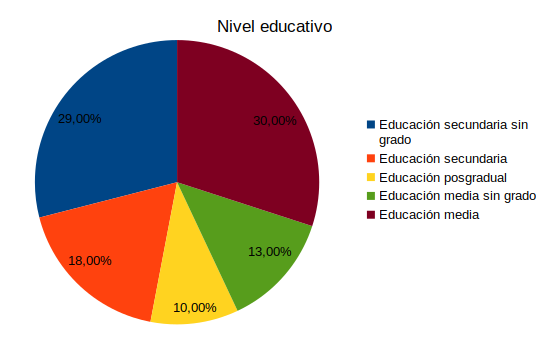
\includegraphics[scale=.45]{Images/Porcentaje.png} 
\item 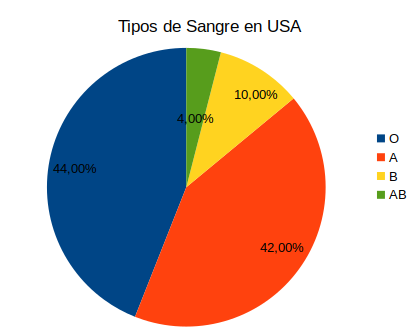
\includegraphics[scale=.45]{Images/TiposSangre.png}
\end{multicols}
\subparagraph*{Repaso:} Encuentre todos los divisores de cada número
\begin{multicols}{2}
\item 84
\item 620
\end{multicols}
\item Encuentre el m.c.m entre 18 y 60
\item Encuentre la descomposición en factores primos de 90
\item Solucione $\frac{5}{8}+y=\frac{13}{16}$
\item Simplifique: $(12-3)^{2}-9+5^{2}$
\end{enumerate}
\end{document}
